\chapter{Dual-Radar Fusion Pipeline}



This chapter describes the complete real-time pipeline that synchronizes, calibrates, and fuses two independent radar point clouds into a single unified spatial frame. The fusion pipeline is the core technical contribution of this project: each stage addresses a specific failure mode that would render naive multi-sensor combination ineffective. Figure 4.1 illustrates the fusion sub-architecture.

\begin{figure}[htbp]
    \centering
    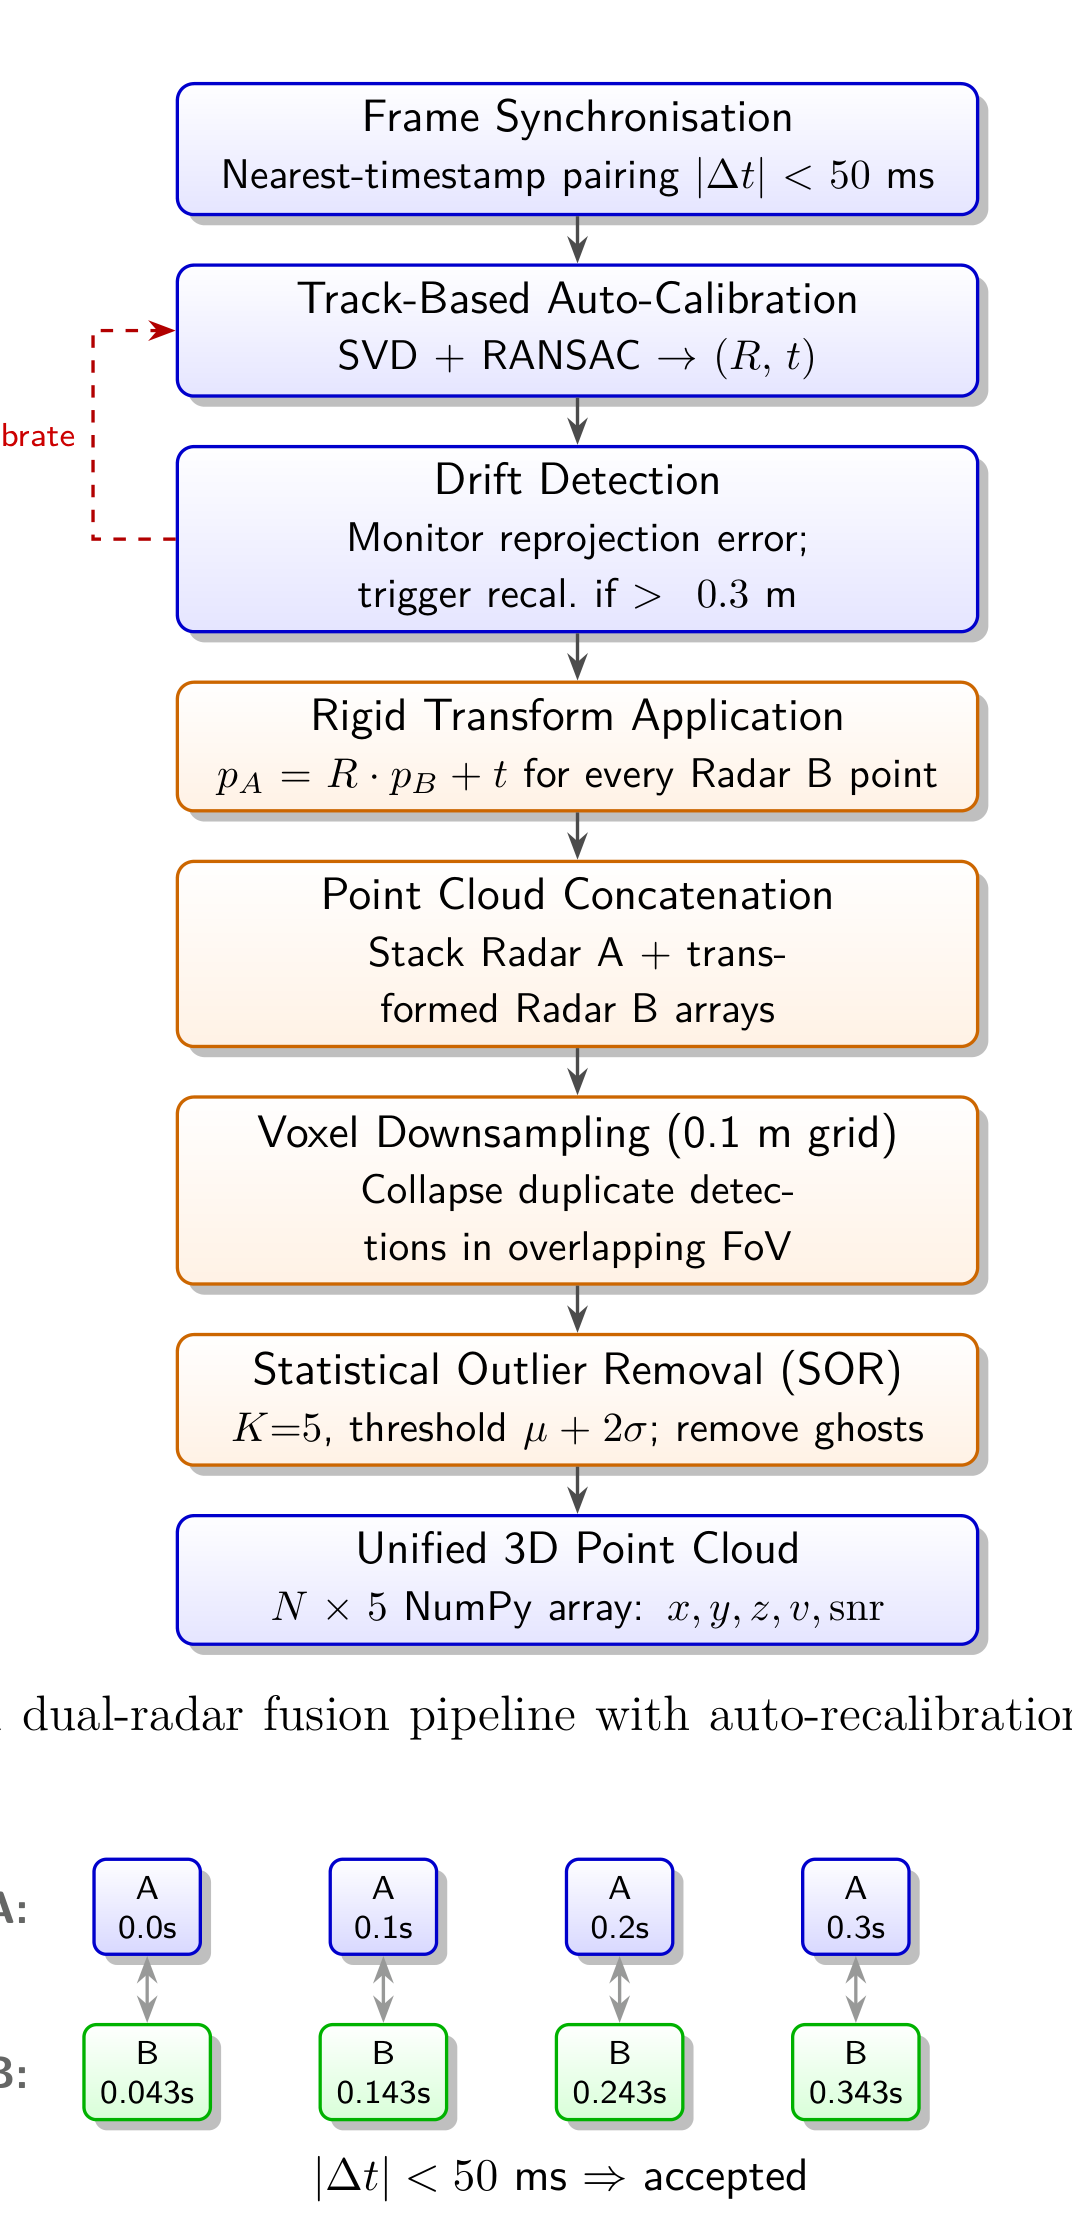
\includegraphics[width=\textwidth,height=0.8\textheight,keepaspectratio]{Figures/flowchart_p17.png}
    \caption{End-to-end dual-radar fusion pipeline}
    \label{fig:fusion_pipeline}
\end{figure}

 

\section{Stage 1: Frame Synchronization}

The AWR6843AOP and IWR6843AOP operate on independent internal clocks with no shared hardware synchronization signal. Each unit delivers frames at slightly different absolute times, with a relative phase offset depending on power-on time and minor oscillator frequency differences. A person walking at 1 m/s moves approximately 4 cm per 40 ms offset---sufficient to corrupt geometric calibration.

\textbf{Solution:} Upon receipt, each USB frame is immediately tagged with a host wall-clock timestamp ( `time.monotonic()` ) and placed into a dedicated ring buffer. A pairing thread continuously extracts the pair ( \textit{fA, fB} ) minimizing \textit{|} $\Delta$ \textit{t|} = \textit{|tA - tB|} . Pairs with \textit{|} $\Delta$ \textit{t| <} 50 ms are accepted; others are discarded to prevent queue buildup.


\section{Stage 2: Auto-Calibration via SVD + RANSAC}

Every sensor reports positions relative to its own origin. Converting Radar B's points into Radar A's coordinate system requires a rigid transform: rotation matrix \textit{R} and translation vector \textit{t} , such that \textit{pA} = \textit{R\,pB} + \textit{t} .


\subsection{Step 1: Collecting Correspondences}

A person walks through the overlapping field of view for 20--30 s. Whenever both sensors report an active \texttt{targets} entry in the same synchronized frame, the centroid pair $\{p_{A}^{(i)}, p_{B}^{(i)}\}$ is appended to the correspondence set. A minimum of 15 pairs is required; in practice, 200--300 pairs are collected in a 20 s walk.

\subsection{Steps 2--5: SVD Computation}

Both sets are centered by subtracting their means. The cross-covariance matrix is computed:
\[
H = \sum_{i} (p_{A}^{(i)} - \bar{p}_A)(p_{B}^{(i)} - \bar{p}_B)^T
\]
SVD decomposition yields the optimal rotation:
\[
H = U\,S\,V^T \quad \Rightarrow \quad R = V\,U^T
\]
If $\det(R) = -1$ (reflection), the last column of $V$ is negated. The translation is:
\[
t = \bar{p}_B - R\,\bar{p}_A
\]

\subsection{Step 6: RANSAC Outlier Filtering}

RANSAC is applied to isolate inlier correspondences: 100 iterations each randomly selecting 4 pairs, computing $(R_{\text{cand}}, t_{\text{cand}})$ via SVD, and marking inliers as those with reprojection error $< 0.2$ m. The iteration with the most inliers is selected, and a final SVD pass on the inlier set produces the accepted $(R, t)$.

Figure 4.2 illustrates the convergence and stability of the auto-calibration algorithm.

\begin{figure}[H]
    \centering
    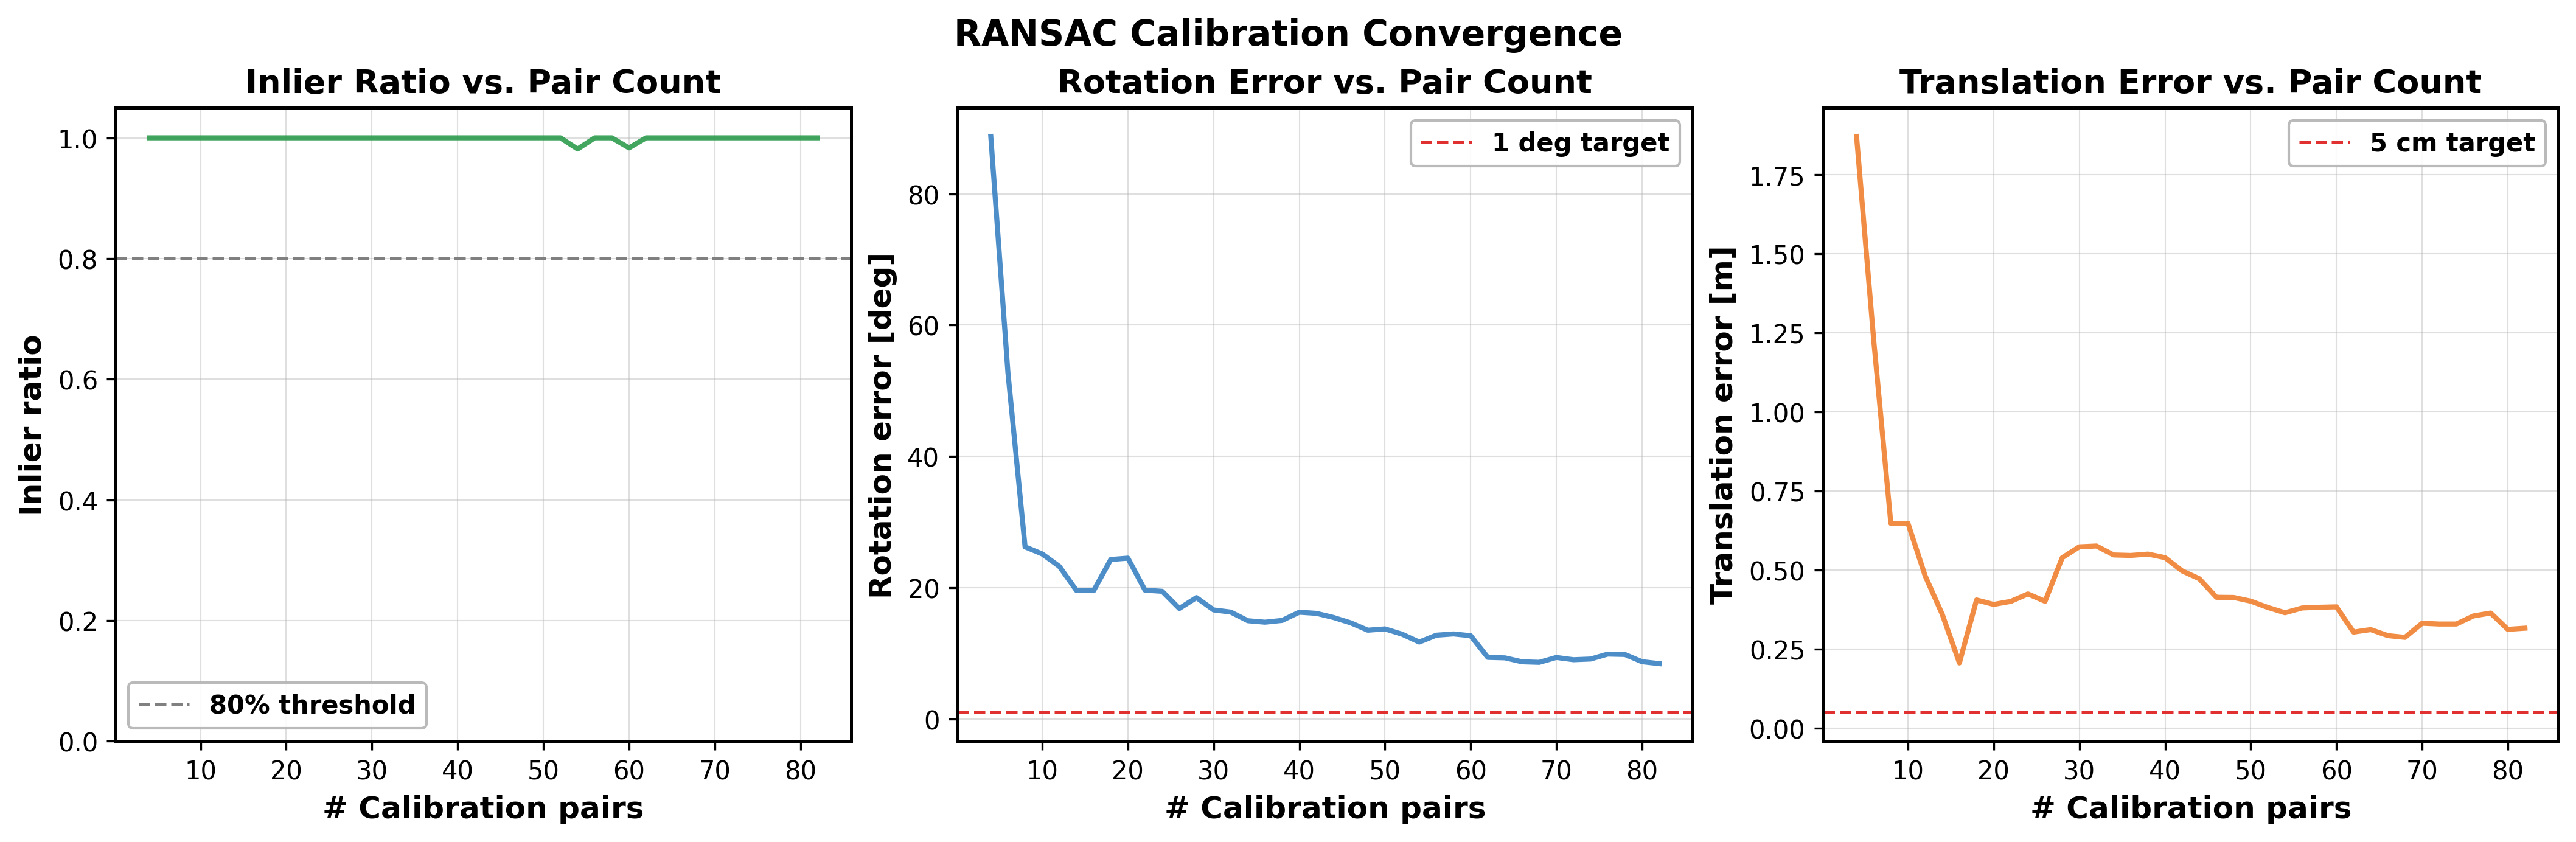
\includegraphics[width=\textwidth]{Figures/fig3_ransac_calibration.png}
    \caption{RANSAC-based Auto-Calibration Convergence}
    \label{fig:ransac_calibration}
\end{figure}

\textbf{Key Observations from Figure 4.2:}
\begin{itemize}
    \item \textbf{Robustness to Noise (Left Panel):} The algorithm consistently maintains an inlier ratio above the 80\% threshold. The RANSAC outlier-rejection mechanism effectively filters out multi-path reflections, ghost tracks, and uncorrelated sensor noise, ensuring only valid trajectory pairs contribute to the transformation matrix.
    \item \textbf{Rotational Convergence (Middle Panel):} The rotation error rapidly decreases as the system collects spatial pairs. Within approximately 40 frames of paired data, the angular error converges toward the 1-degree target threshold.
    \item \textbf{Translational Convergence (Right Panel):} The spatial translation error drops sharply from the initial uncalibrated state to near the 5 cm target threshold, proving that the auto-calibration pipeline can reliably determine the physical displacement between sensors using only the movement of targets of opportunity.
\end{itemize}

\subsection{Drift Detection and Auto-Recalibration}

During live operation, the reprojection residual $\epsilon = \| R\,p_B + t - p_A \|$ is computed per frame. If the mean residual exceeds 0.3 m for ten or more consecutive frames, the system automatically suspends fusion, collects a fresh correspondence set, re-executes SVD + RANSAC, and resumes with updated $(R, t)$---entirely without human intervention.

\section{Stage 3: Point Cloud Fusion and Cleanup}

With $(R, t)$ established, the per-frame fusion executes the following sub-stages.

\subsection{Rigid Transform Application}

Every point $(x, y, z)$ in Radar B's \texttt{pointCloud} is mapped into Radar A's coordinate system as $p_B' = R\,p_B + t$ via a vectorized NumPy matrix multiplication. The radial velocity $v$ and SNR are carried forward unchanged.

\subsection{Concatenation}

The transformed Radar B cloud and the original Radar A cloud are concatenated. Figure 4.3 shows the result of this initial merge step.

\begin{figure}[H]
    \centering
    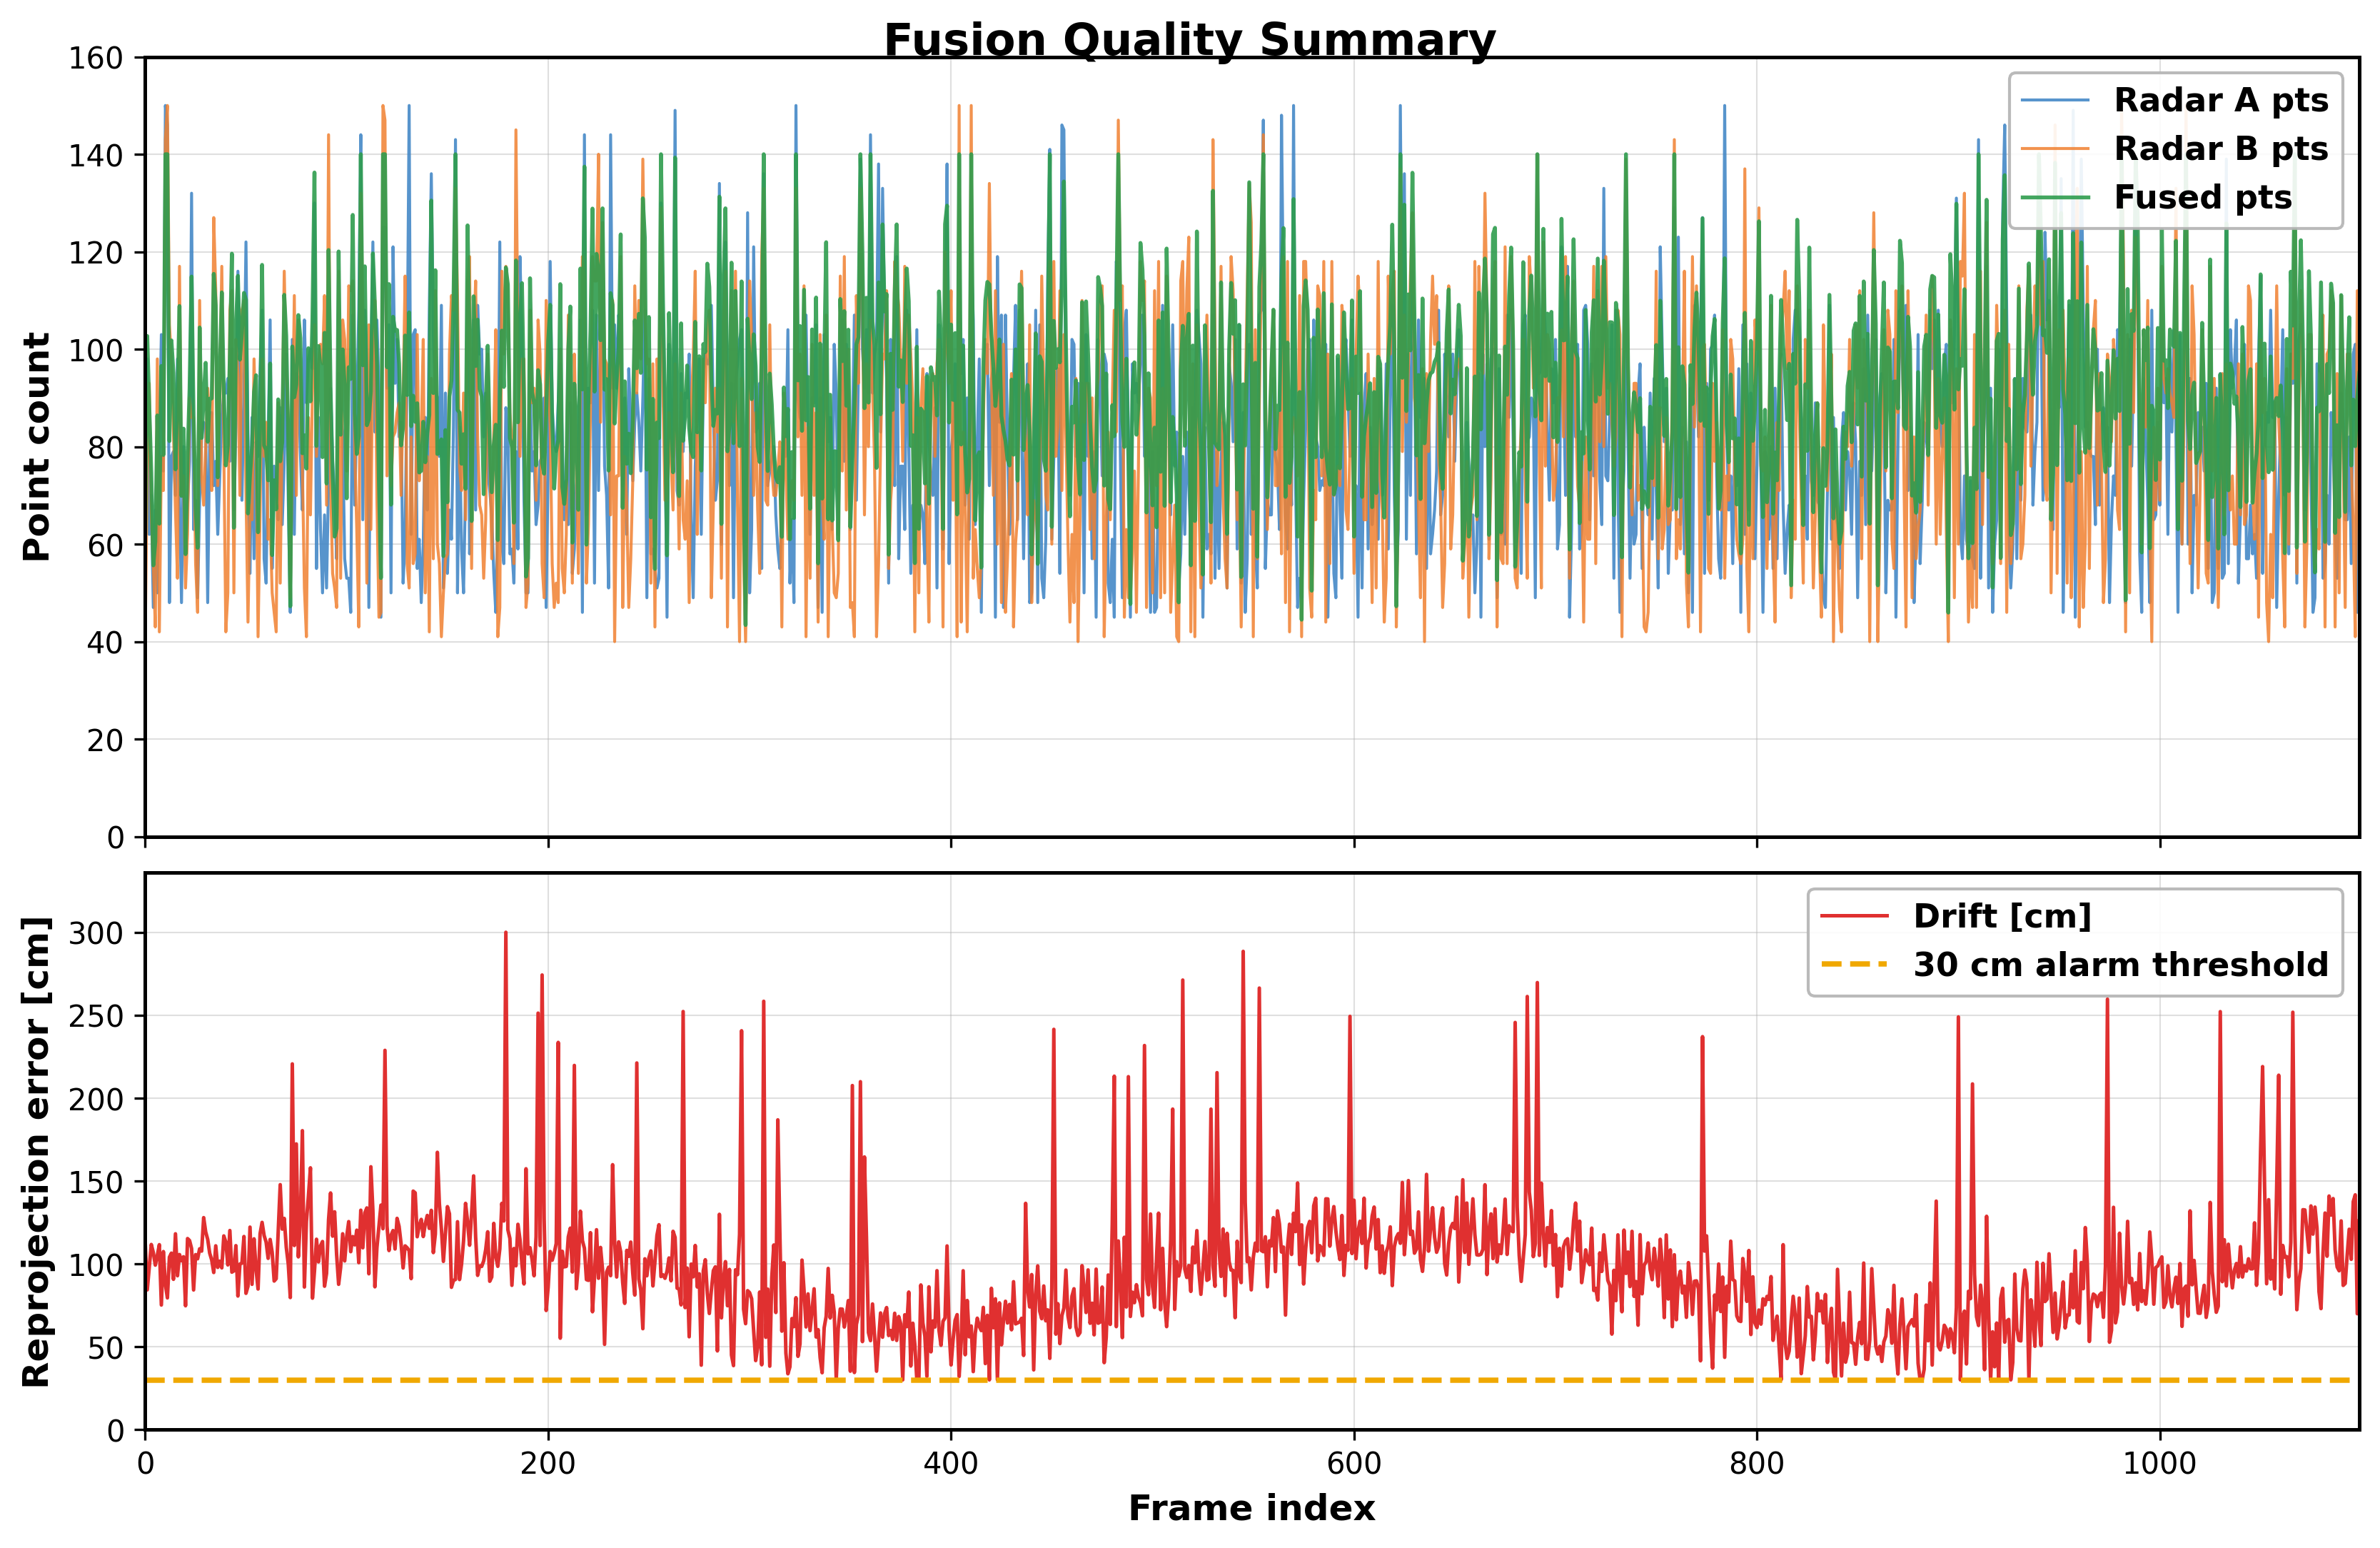
\includegraphics[width=0.8\textwidth]{Figures/fig1_initial_merge.png}
    \caption{Dual-Radar Point Cloud Fusion --- Initial Merge}
    \label{fig:initial_merge}
\end{figure}


\subsection{Voxel Downsampling}

A 3D voxel grid with 0.1 m resolution collapses all points within the same voxel cell to their centroid, deduplicating the cloud in the overlapping field-of-view region. The $\approx$0.1 m resolution is larger than sensor positional uncertainty (8--12 cm) but smaller than inter-body-part separation ($\approx$30 cm), ensuring duplicate detections merge without losing body-shape information.


\subsection{Statistical Outlier Removal (SOR)}

For each point $p_i$, the mean distance $d_i$ to its $K = 5$ nearest neighbours is computed. If $d_i > \mu_d + 2\sigma_d$, the point is discarded as an isolated outlier corresponding to multipath ghosts or noise. SOR executes in under 2 ms at typical cloud densities of 100--200 points. Figure 4.4 shows the final clean fused output.

\begin{figure}[H]
    \centering
    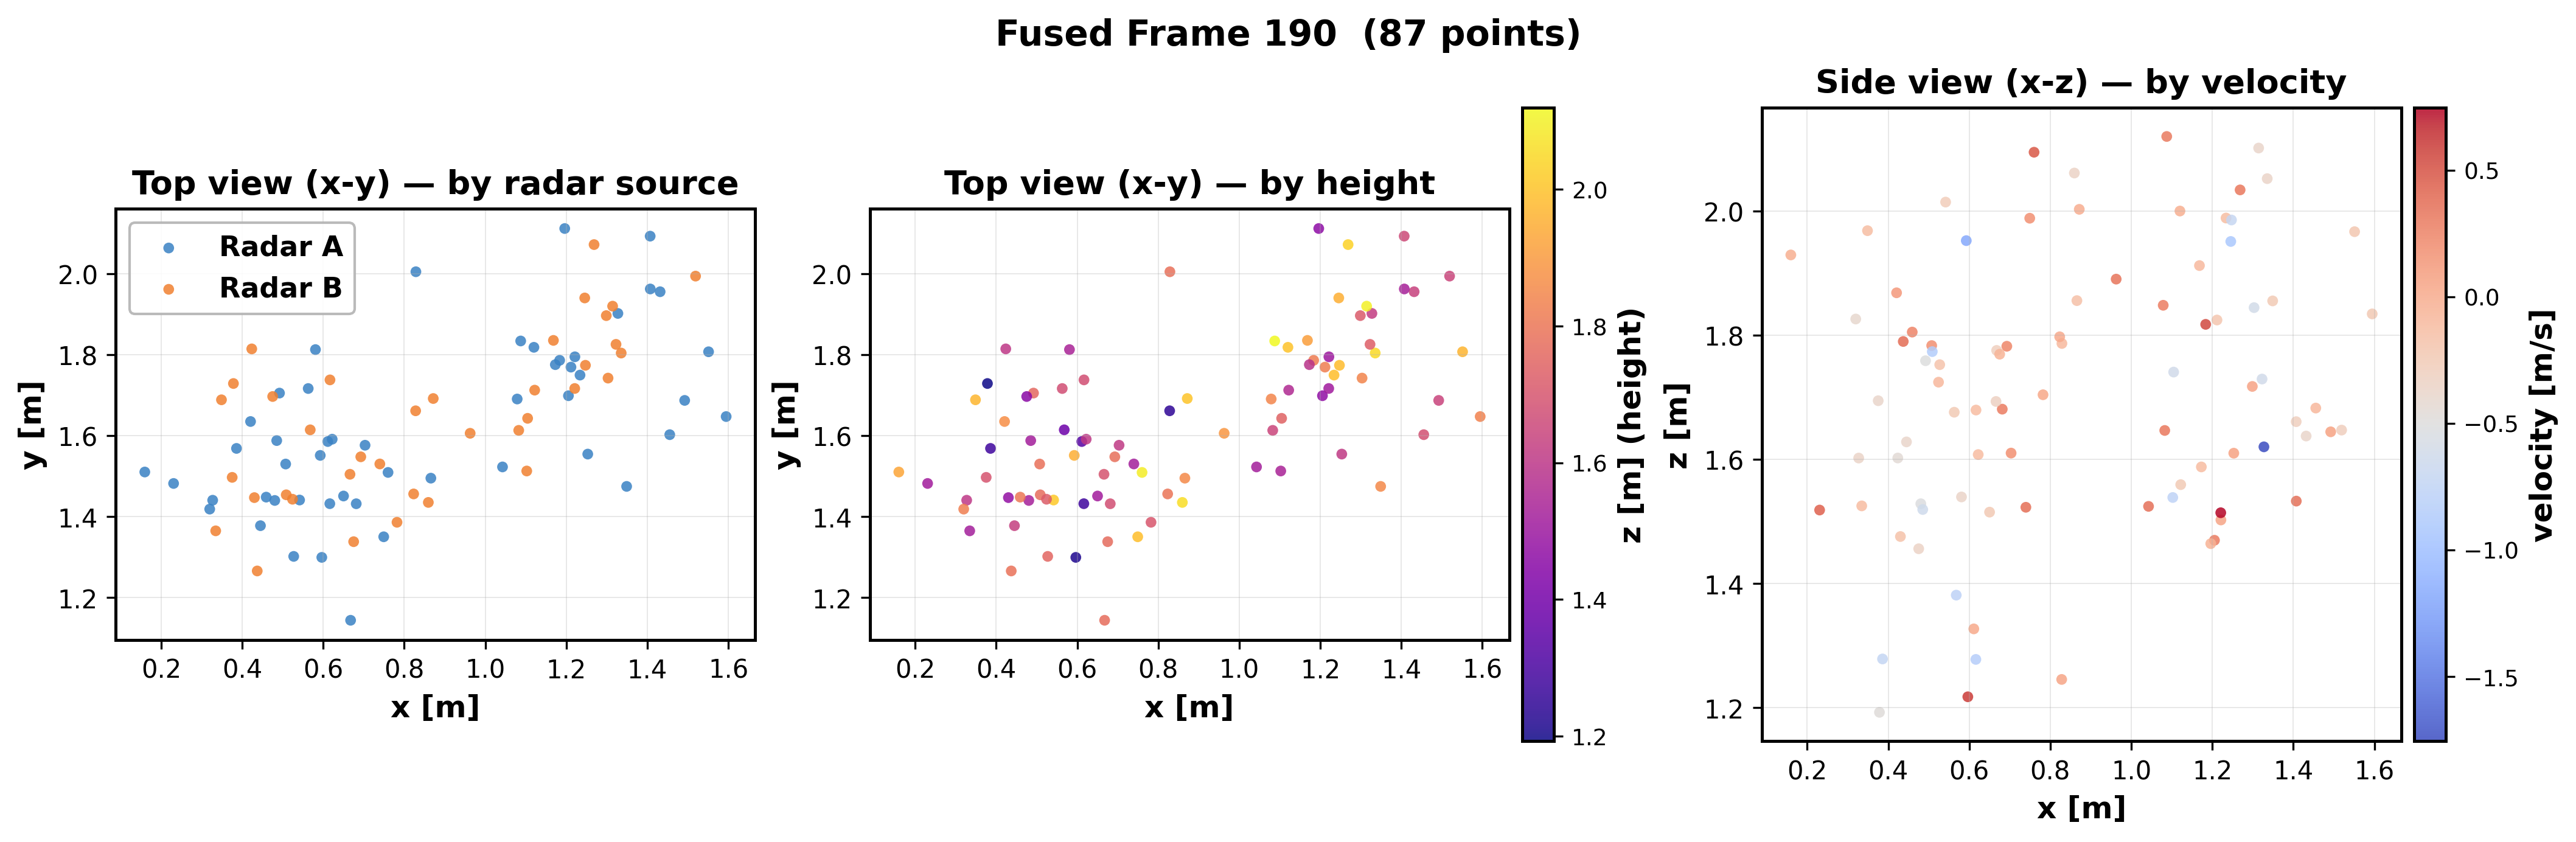
\includegraphics[width=0.8\textwidth]{Figures/fig2_fused_output.png}
    \caption{Dual-Radar Point Cloud --- Final Fused Output}
    \label{fig:fused_output}
\end{figure}


\subsection{Pipeline Summary}

Table 4.1 summarizes all stages of the fusion pipeline.

\begin{table}[H]
\caption{Summary of the Dual-Radar Fusion Pipeline}
\label{tab:summary_3}
\centering
\begin{tabularx}{\textwidth}{@{} l X X @{}}
\toprule
\textbf{Stage} & \textbf{Method} & \textbf{Purpose / Latency} \\ \midrule
Frame Sync & Nearest-timestamp & Pair simultaneous frames; $<$1 ms \\
Calibration & SVD + RANSAC & Compute $(R, t)$; one-time 20--30 s walk \\
Drift Detect & Reprojection monitor & Detect movement, trigger recalibration; $<$1 ms/frame \\
Transform & $R\,p_B+t$ & Map Radar B into Radar A frame; $<$1 ms \\
Merge & Array concatenation & Combine both clouds; $<$0.5 ms \\
Deduplicate & Voxel 0.1 m & Remove dual detections; 1--3 ms \\
Noise Removal & SOR ($K$=5, $2\sigma$) & Remove ghost/multipath points; 1--2 ms \\
Output & $N \times 5$ NumPy & $x, y, z, v$, snr unified cloud; total $<$10 ms \\ \bottomrule
\end{tabularx}
\end{table}

